\chapter{Related Work}
\label{c:related_work}

This chapter surveys previous work in the domain of cloud-of-clouds and distinguishes FileFarm from these efforts. To preserve data confidentiality and avoid service availability failure caused by dependence on a single cloud, research related to cloud-of-clouds, or in other words, "multi-clouds" or "interclouds", has emerged and received increasing attention. Generally speaking, the main goal of cloud-of-clouds research is to seek a reliable and cost-efficient way to disperse data across multiple cloud providers and avoid dependence or data leakage on any of them. Indeed, an adequate cloud-of-clouds design needs to take a wide variety of aspects into consideration. To make a clear comparison among these efforts, we arrange this chapter into several sections, each discussing an important aspect to be considered and the corresponding mechanisms employed by each work. In the end of each section, we demonstrate the approach adopted by FileFarm and explain the differences between FileFarm and other cloud-of-clouds works.

\begin{table}[!b]
\centering
  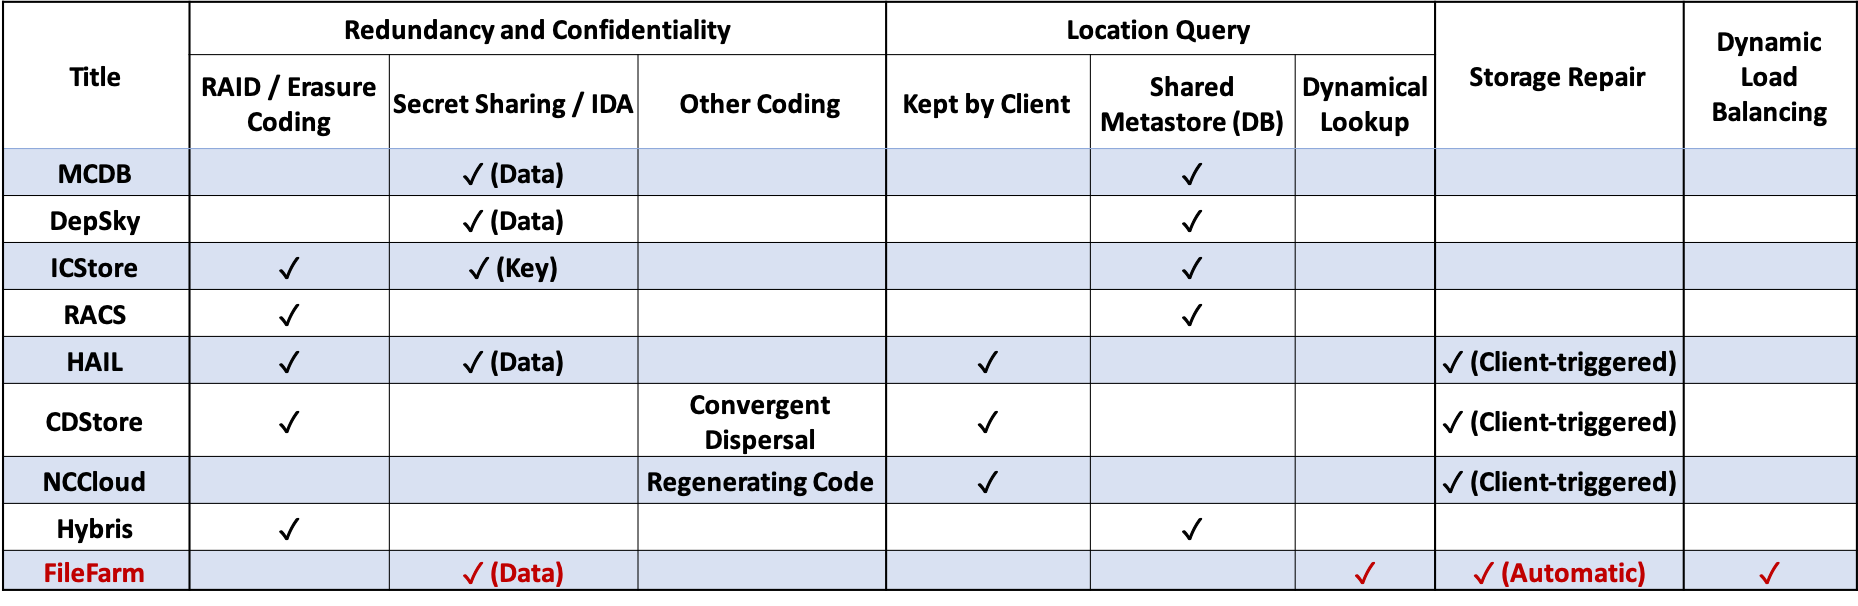
\includegraphics[width=15cm]{tables/table_property_comparison.png}
  \caption{Comparison of properties provided by related cloud-of-clouds designs}
  \label{table:propertycomparison}
\end{table}

% redundancy and confidentiality
\section{Redundancy and Confidentiality}
\label{ss:cocredundancyandconfidentiality}

To avoid dependence of data retrievability on a single cloud, redundancy mechanisms need to be introduced into design of cloud-of-cloud systems. To provide redundancy, RACS\cite{abu2010racs} and HAIL\cite{bowers2009hail} claim their approaches as RAID-like techniques used by disks and file systems, but at the cloud service level. By striping data across multiple providers, RAID-like approach helps customers to avoid vendor lock-in, reduce the cost of switching providers, and better tolerate provider outages or failures. The same benefits can also be provided by erasure coding, which is implemented in ICStore\cite{cachin2010dependable}, CDStore\cite{li2015cdstore} and Hybris\cite{dobre2014hybris}. In fact, RAID-like and erasure coding approaches do not differ too much from each other in the cloud context, considering the fact that cloud storage services usually provide simple key/value store APIs but not a fully functional disk; thus the RAID-like approach does not literally works like an array of pre-allocated storage spaces. Instead, it is more reasonable to view it as an array of redundant data chunks stored on different clouds, which is in the same sense as the erasure coding mechanism.

Besides erasure coding, secret sharing mechanisms such as Shamir's Secret Sharing\cite{shamir1979share} and Information Dispersal Algorithm\cite{rabin1989efficient} also provides redundancy as their side benefit. These mechanisms splits a piece of data into several, say $n$, encrypted chunks, with the assurance that a certain number $m <= n$ of these encrypted chunks are sufficient for recovering the original data. Thus, these secret sharing mechanisms provide advantages in both redundancy and confidentiality. The mechanisms are employed by MCDB\cite{alzain2011mcdb}, DepSky\cite{bessani2013depsky}, ICStore\cite{cachin2010dependable}, HAIL\cite{bowers2009hail}, and also FileFarm.

There are still some other coding mechanisms designed` to provide redundancy and confidentiality for cloud-of-cloud storage. For instance, CDStore\cite{li2015cdstore} is built on an augmented secret sharing schema called convergent dispersal, which provides benefits of de-duplication, storage savings and robustness against side-channel attacks. NCCloud\cite{hu2012nccloud} use functional minimum storage regenerating code (F-MSR) to achieve cost-effective repair for a permanent single-cloud failure.

% location query
\section{Location Query}
\label{ss:coclocationquery}

In a cloud-of-clouds storage system, each data chunk is distributed over some (but not all) of the clouds. To store files and retrieve them back successfully and efficiently, the system must define a way for clients to query which clouds their files are stored on, which we call \textit{location query}. Systems like HAIL\cite{bowers2009hail}, CDStore\cite{li2015cdstore}, NCCloud\cite{hu2012nccloud} focus more on retrievability and algorithms of dispersal while emphasizing less on this part. From these works, we can only inferred that location information is either kept by clients or managed by other layers that are integrated with these systems.

Systems like MCDB\cite{alzain2011mcdb}, DepSky\cite{bessani2013depsky}, ICStore\cite{cachin2010dependable}, RACS\cite{abu2010racs}, Hybris\cite{dobre2014hybris} address another solution to location query. In these systems, location information is stored on a shared \textit{metastore}, which is implemented in the form of a database or a simple key/value store. By applying the metastore design, clients in these systems can efficiently get acknowledged of the clouds from which they can download data, within one or few database queries. This provides a convenient and strait-forward way for clients to access their data. Besides, since meta information is stored separately from data, the risk of malicious insider threats on clouds can be reduced significantly. For instance, Hybris\cite{dobre2014hybris} advocates a hybrid cloud structure in which meta data are stored on trusted premises of private servers while encrypted data chunks are stored on untrusted public clouds. With such trust-boundary design, Hybris leverages strong consistency of meta data stored off-clouds to mask the weak consistency of data stored in clouds.

Nevertheless, there are several issues related to such metastore designs. First, since the mapping between files and clouds is saved as static database records, the records will become out-of-date if some clouds encounter service outage, which has a direct impact on retrievability of files. Second, the static approach has a lack of mechanisms for dynamical replication of shard when encountering permanent single-cloud failures. As a result, the systems have low tolerance for less-reliable providers or successive changes of clouds over a long period of time. Third, considering the cases of new clouds joining the system, it takes high cost to re-distribute the data over all clouds; thus these systems would suffer from load-balancing issues and high vendor-switching cost inevitably. Last but not the least, the metastore is regarded as a logically-centralized layer. In spite of the fact that this layer might be implemented with Byzantine Fault Tolerance algorithms or distributed synchronization tools (e.g. Apache ZooKeeper\cite{zookeeper}), the system cannot work without this layer, which means any fault occurring to this layer will pose an direct impact on the whole system.

To solve the problems caused by a logically-centralized metastore layer, FileFarm adopts a distributed approach for location query. In FileFarm, clouds coordinate with each other to form a peer-to-peer storage network, while data chunks can be located with an efficient and dynamical lookup procedure defined by Kademlia\cite{maymounkov2002kademlia} DHT protocol. Without a centralized layer storing static information, location query mechanism in FileFarm does not suffer from out-of-date issue and is robust to churn of clouds and network changes in terms of topology or scale. This is the fundamental difference between FileFarm and traditional cloud-of-clouds approaches. Based on this architectural difference, FileFarm is able to carry out more features that can not be handled well by centralized or hierarchical solutions, such as automatic storage repair, load-balancing, and better degree of fault tolerance.

% storage repair
\section{Storage Repair}
\label{ss:cocstoragerepair}

An important property of cloud-of-clouds systems is disaster recovery. To be specific, when a cloud encounters service failure, the redundancy of each data chunk it used to stored is reduced by a certain factor. To maintain consistent level of redundancy, a \textit{storage repair} mechanism needs to be included in the cloud-of-clouds system design. For an erasure coding based system, an instinctive approach toward storage repair is to let clients download sufficient chunks of data back, reconstruct the lost chunk, and then re-distribute it to other clouds. This is the exact approach implemented by HAIL\cite{bowers2009hail} and CDStore\cite{li2015cdstore}. In fact, this is a general procedure of storage repair that can be employed to all coding-based redundancy schemas, while not explicitly described by some of the related implementations. Besides the general procedure described above, some systems meet requirements of storage repair with different coding mechanism, seeking to reduce the repair traffic. For instance, NCCloud\cite{hu2012nccloud} uses network coding based schema to maintain the same data redundancy level as erasure codes, but uses less repair traffic.

While the download-and-redistribute approach manages to repair storage failure and preserve consistent level of redundancy, it is considered to be unfeasible for one primary reason: the mechanism requires \textit{clients} to detect and trigger the entire storage repair procedure manually, which violates the design pattern of cloud services where service reliability should be maintained by the service provider internally and should not rely on any action of clients.

To address this issue, FileFarm adopts a different approach toward storage repair by leveraging its distributed nature. In FileFarm, each stored chunk of data is "re-published" by exactly one storage node in a period of time. As public clouds are considered to be robust, the period can be set long, say, one month. When a cloud encounters service failure, the republish mechanism will repair redundancy automatically within the following one period, without any involvement of other parties required. The same mechanism also offers benefits of load-balancing when new clouds join the network, which will be explained in \ref{ss:storagerelease}. The automatic load-balancing and storage repair properties also make a clear distinction of FileFarm from other cloud-of-clouds works.

% MCDB: use secret-sharing algorithm to avoid the risk of malicious insiders in the cloud and to avoid the failing of cloud services. 


% DepSky: using an efficient set of Byzantine quorum system protocols, cryptography, secret sharing, erasure codes and the diversity that comes from using several clouds.


% ICStore: ICStore client consists of three core layers that target different dependability aspects: i) confidentiality, ii) integrity and iii) reliability and consistency (RC). This layered approach allows individual layers to be switched “on” and “off” to provide different levels of dependability that are to be matched with client’s goals, also with performance and possibly even monetary constraints in mind. In addition, each layer can be individually tuned, as we detail in the following.


% RACS: applying RAID-like techniques used by disks and file systems, but at the cloud storage level. We argue that striping user data across multiple providers can allow customers to avoid vendor lock-in, reduce the cost of switching providers, and better tolerate provider outages or failures


% HAIL: manages file integrity and availability across a collection of servers or independent storage services. It distributes data blocks over servers with information dispersal algorithm and makes use of PORs as building blocks by which storage resources can be tested and reallocated when failures are detected.


% CDStore: builds on an augmented secret sharing schema called convergent dispersal, which supports de-duplication by using deterministic content-derived hashes as inputs to secret sharing. achieve both bandwidth and storage savings and be robust against side-channel attacks.

% NCCloud: use regenerating codes to achieve cost-effective repair for a permanent single-cloud failure. propose an implementable design for the functional minimum- storage regenerating code (F-MSR), which maintains the same data redundancy level and same storage requirement as in traditional erasure codes (e.g., RAID-6), but uses less repair traffic.


% Hybris: Hybris disperses data (using replication or erasure coding) across multiple untrusted and possibly inconsistent public clouds, while it replicates metadata within trusted premises of a private cloud. Hybris tolerates up to f arbitrary public cloud faults and is very efficient: in the common-case (with replicated variant of Hybris), writes accesses only f + 1 clouds, while a reads accesses a single, “closest” cloud. In a sense, Hybris is the first multi-cloud storage protocol that makes it possible to tolerate potentially malicious clouds at the price of tolerating simple cloud outages. To complement this, Hybris offers strong consistency as it leverages strong consistency of metadata stored offclouds to mask the weak consistency of data stored in clouds.

